\documentclass{article}
\usepackage{amsmath}
\usepackage{amssymb}
\usepackage{multirow}
\usepackage{graphicx}
\usepackage{kotex}
\author{lichen}
\date{\today}
\begin{document}
    \section{실험 설계 개요}
    주어진 실험 계획에서 4개 요소에서 (DMEM 농도, 미세조류 추출물 농도, 성장인자 1 농도, 성장인자 2 농도)
    FBS 농도 최소화, 세포 증식률 최대화 조건 탐색 
    $3*4*4*4*4 = 768$가지 조합을 실험해봐야 함.\\
    FBS 농도에 따라 Table \ref{table1}과 같이 Block을 설정함. 각 Block은 Table \ref{table2}에서 요소별 수준 조합으로 실험을 진행함.
    이 경우 필요한 실험의 수는 $4*\text{Block 별 실험 수}$임.
    \begin{table}[h]
        \centering
        \begin{tabular}{|c c c c|}
            \multicolumn{4}{|c|}{FBS 농도}\\
            \hline
            0 & 0.5 & 1 & 2\\
            Block1 & Block2 & Block3 & Block4\\
        \end{tabular}
        \caption{ FBS 농도별 Block 설정}
        \label{table1}
    \end{table}
    \begin{table}[h]
        \centering
        \begin{tabular}{|c c c c c|}
            요소&\multicolumn{4}{|c|}{수준}\\
            \hline
            DMEM &  & 0.5 & 0.75 & 1 \\
            미세조류 추출물 & 0 & 2 & 4 & 6 \\
            성장인자 1 & 0 & 5 & 10 & 15 \\
            성장인자 2 &  0 & 5 & 10 & 15 \\ 
        \end{tabular}
        \caption{ Block 설정}
        \label{table2}
    \end{table}
    \newpage
    \section{Block의 실험 설계}
    Block 별 실험 수를 최소화하기 위해 다음과 같은 방법을 시도할 수 있음.
    \begin{itemize}
        \item 선별 반응설계 : 2 수준 별 요소를 중복없이 조합하여 실험을 진행함.\\
        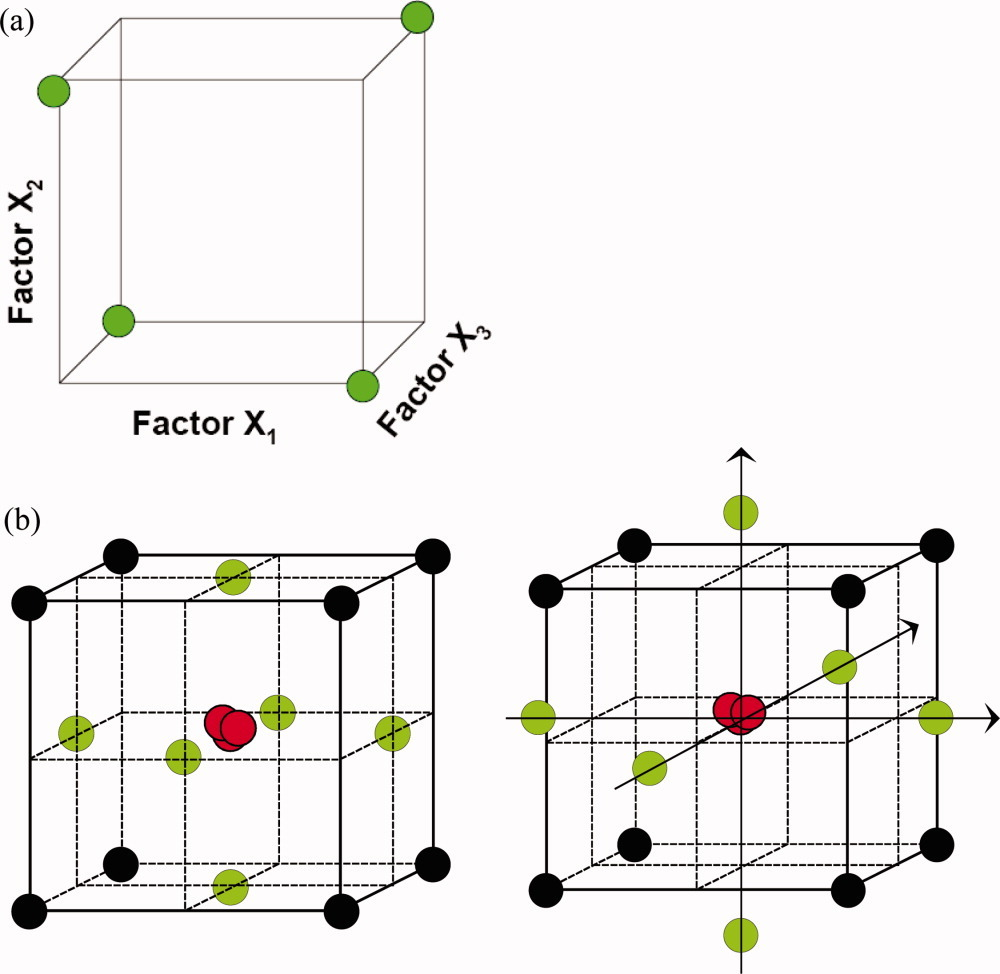
\includegraphics[scale=0.3]{fatorial design.jpg}
        \item 반응표면실험 : 연속형 요인의 양 구간 끝과 중점을 조합하여 실험을 진행함. \\
        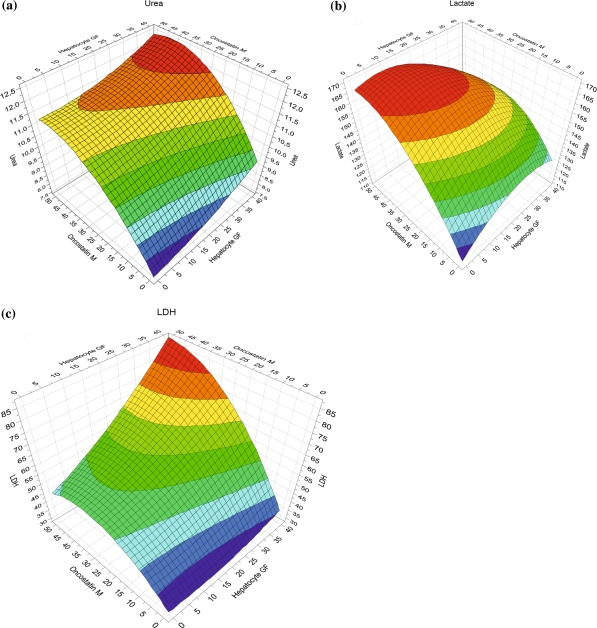
\includegraphics[scale=0.3]{reactionsurfae.jpg}
    \end{itemize}
    \section{minitab을 이용한 실험 설계}
    minitab은 웹에서 이용가능. 
    부분 요인설계, 다수준 요인설계, Box-Benheken 설계 진행함.\\
    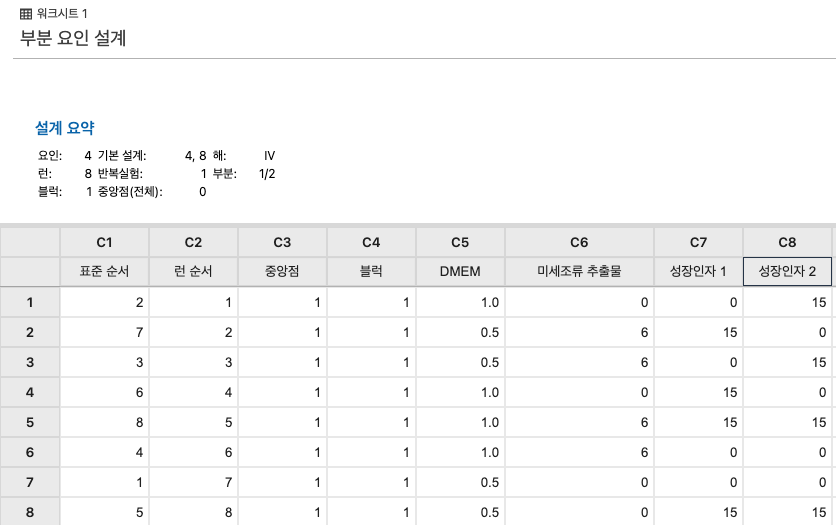
\includegraphics[scale=0.5]{min3.png}
    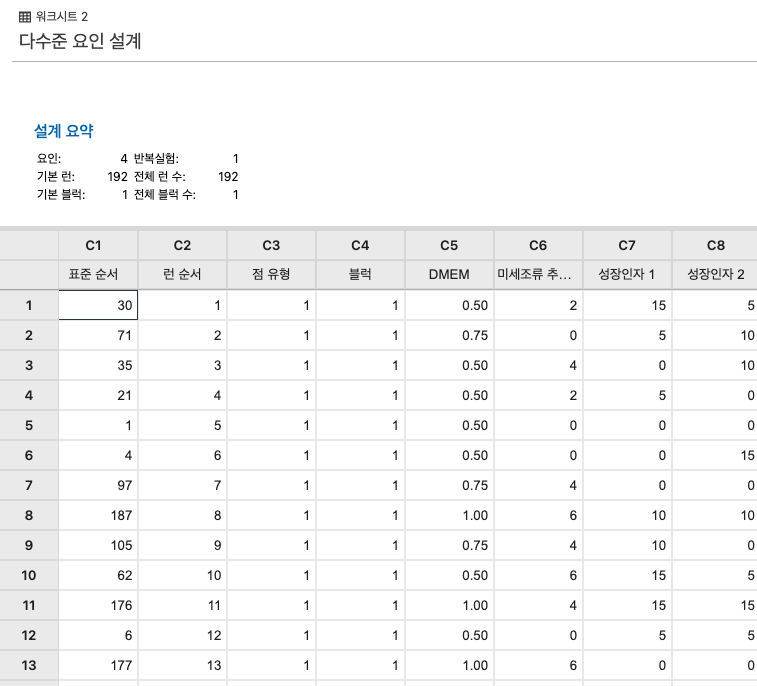
\includegraphics[scale=0.5]{min2.png}
    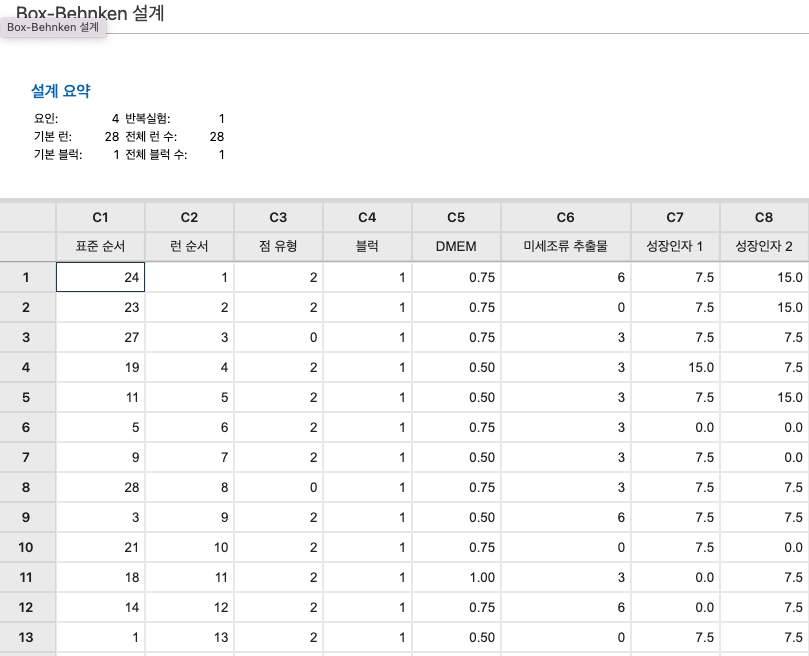
\includegraphics[scale=0.5]{box-behnken.png}
    \section{JMP를 이용한 실험 설계}
    부분 요인설계, Box-Benheken 설계 진행함.\\
    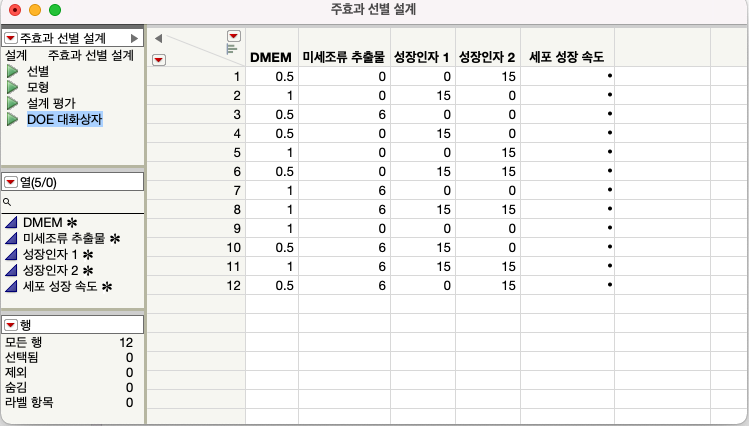
\includegraphics[scale=0.5]{jmp2level.png}\\
    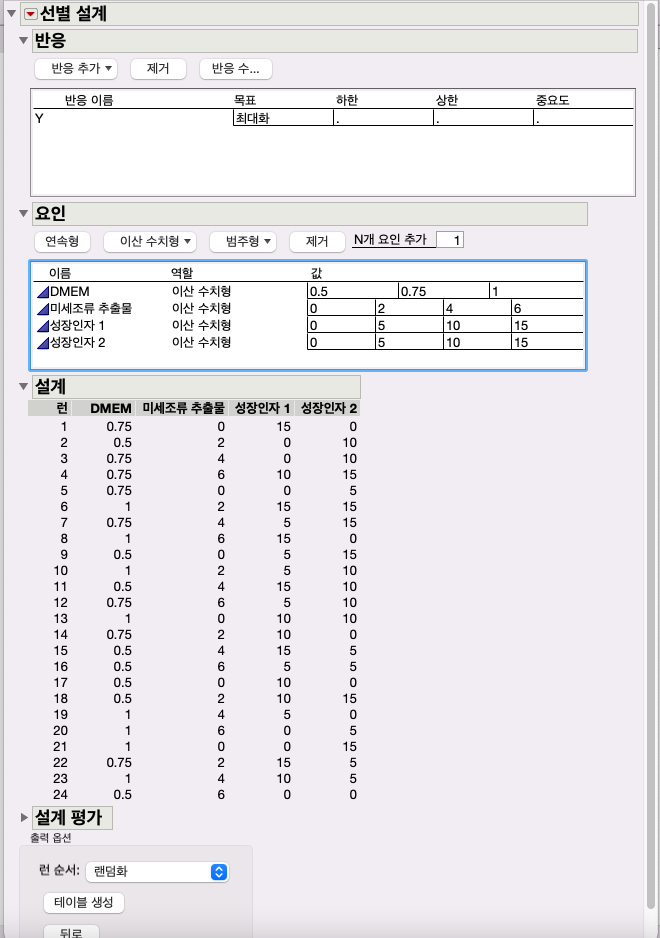
\includegraphics[scale=0.5]{jmpdescretic.png}\\
    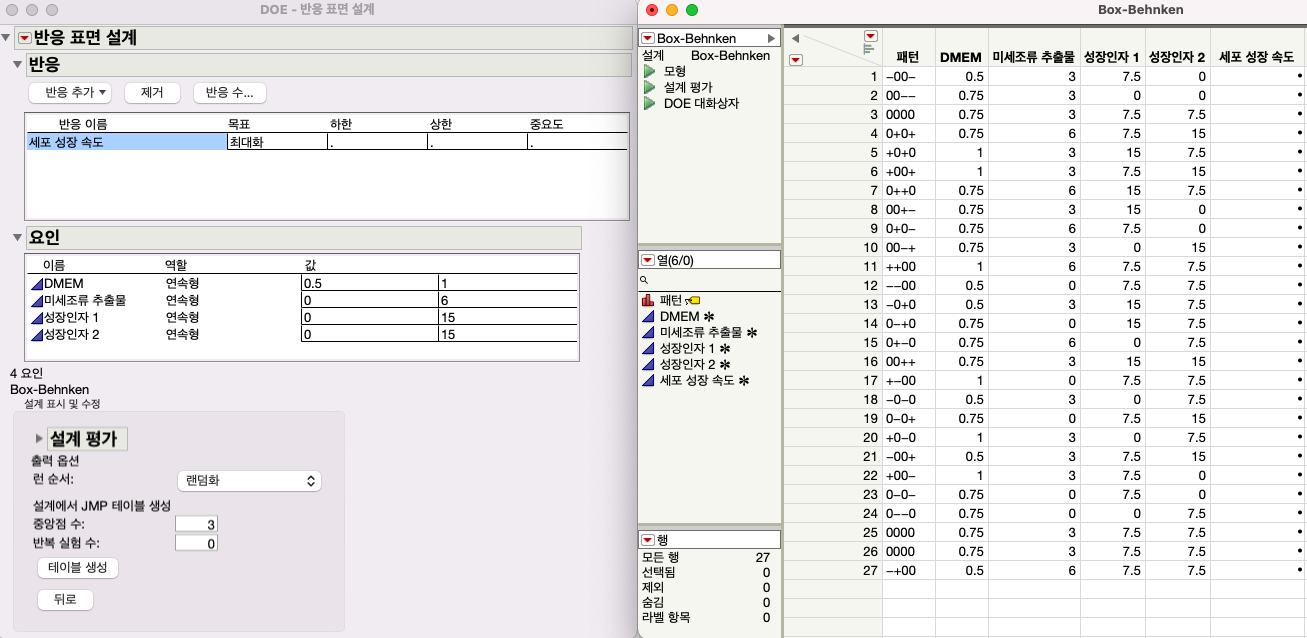
\includegraphics[scale=0.3]{boxbenhken.png}
    \section{결론}
    \begin{itemize}
        \item JMP가 minitab에 비해 더 많은 설계 옵션 제공
        \item 동일한 실험 설계에 대해서는 프로그램 관계 없이 동일한 결과 제공
        \item 현재 실험 수준에서는 오픈 소스 사용으로 실험 설계 및 분석 대체 가능함
    \end{itemize}
\end{document}